\documentclass[english]{beamer}
\usepackage{makeidx}
\usepackage{color}
\usepackage{graphicx}
%\usepackage[pdftex]{graphicx}
\usetheme{Goettingen}
\setbeamercovered{transparent}

\usenavigationsymbolstemplate{}

\definecolor{ListingBorderColor}{gray}{0.55}
\definecolor{ListingBackgroundColor}{gray}{0.95}

\usepackage{babel}
\usepackage{hyperref}
\usepackage{enumerate}
\usepackage{enumerate}
\usepackage{longtable}
\usepackage[T1]{fontenc}
\usepackage{ucs}
\usepackage[latin1]{inputenc}
\usepackage{textcomp}
\usepackage{alltt}
\usepackage{listings}
\usepackage{fancyvrb}

\title{Git Basics}
\author[Bart Trojanowski, Sonia Hamilton]
{Bart Trojanowski \href{mailto:bart@jukie.net}{bart@jukie.net}\\
This edit {Sonia Hamilton \href{mailto:sonia@snowfrog.net}{sonia@snowfrog.net}}}
\institute{Jukie Networks Inc.}
\date{31st August, 2012}

\newcommand{\mysection}[2]{%
  \hypertarget{#2}{}%
  \section{#1}%
  \label{#2}%
}
\newcommand{\mysubsection}[2]{%
  \hypertarget{#2}{}%
  \subsection{#1}%
  \label{#2}%
}

\definecolor{code-black}{rgb}{0,0,0}
\definecolor{code-green}{rgb}{0,0.3,0}
\definecolor{code-orange}{rgb}{0.4,0.3,0}
\definecolor{code-blue}{rgb}{0,0,0.5}
\definecolor{code-red}{rgb}{0.7,0,0}
\definecolor{code-gray}{rgb}{0.7,0.7,0.7}
\definecolor{code-white}{rgb}{1,1,1}
\newcommand{\ttt}[1]{%
\texttt{\textcolor{code-black}{#1}}%
}
\newcommand{\CMD}[1]{%
\texttt{\textcolor{code-green}{#1}}%
}
\newcommand{\cmd}[1]{%
\texttt{\textcolor{code-orange}{#1}}%
}
\newcommand{\gui}[1]{%
\texttt{\textcolor{code-blue}{#1}}%
}
\newcommand{\err}[1]{%
\texttt{\textcolor{code-red}{#1}}%
}
\newcommand{\fnt}[1]{%
\texttt{\textcolor{code-gray}{#1}}%
}
\newcommand{\hide}[1]{%
\texttt{\textcolor{code-white}{#1}}%
}

\newcommand{\black}[1]{%
\textcolor{code-black}{#1}%
}
\newcommand{\faint}[1]{%
\textcolor{code-gray}{#1}%
}
\newcommand{\green}[1]{%
\textcolor{code-green}{#1}%
}
\newcommand{\blue}[1]{%
\textcolor{code-blue}{#1}%
}
\newcommand{\red}[1]{%
\textcolor{code-red}{#1}%
}

\begin{document}
% =====================================================================
\label{header}\hypertarget{header}{}
\frame{\maketitle}

% =====================================================================
% =====================================================================
\mysection{Concepts}{_concepts}
% =====================================================================
\mysubsection{Decentralization}{concepts:decentralization}

% ---------------------------------------------------------------------
\begin{frame}
\frametitle{Centralized SCM - Subversion}
\includegraphics[width=\linewidth]{centralized.eps}
\begin{itemize}
        \item operations require \textcolor{red}{server}
                \begin{itemize}
                        \item single point of failure
                        \item bottleneck
                \end{itemize}
\end{itemize}
\end{frame}

% ---------------------------------------------------------------------
\begin{frame}
\frametitle{Decentralized SCM}
\includegraphics[width=\linewidth]{decentralized.eps}
\begin{itemize}
        \item anyone can be a server
\end{itemize}
\end{frame}

% ---------------------------------------------------------------------
\begin{frame}
\frametitle{Structure}

\includegraphics[width=\linewidth]{struct-02.eps}
\vspace{\baselineskip}
\begin{center}
        the three 'areas'
\end{center}
\vspace{\textheight}
\end{frame}

% ---------------------------------------------------------------------
\begin{frame}
\frametitle{Structure}

\includegraphics[width=\linewidth]{struct-03.eps}
\vspace{\baselineskip}
\begin{center}
        ``staging''

        \vspace{\baselineskip}
        \CMD{add} \\
        \CMD{remove} \\
        \CMD{rename}
\end{center}
\vspace{\textheight}
\end{frame}

% ---------------------------------------------------------------------
\begin{frame}
\frametitle{Structure}

\includegraphics[width=\linewidth]{struct-04.eps}
\vspace{\baselineskip}
\begin{center}
        ``committing''

        \vspace{\baselineskip}
        \CMD{commit}
\end{center}
\vspace{\textheight}
\end{frame}

% ---------------------------------------------------------------------
\begin{frame}
\frametitle{Structure}

\includegraphics[width=\linewidth]{struct-05.eps}
\vspace{\baselineskip}
\begin{center}
        ``reading tree''

        \vspace{\baselineskip}
        \CMD{checkout} \\
        \CMD{reset}
\end{center}
\vspace{\textheight}
\end{frame}

% ---------------------------------------------------------------------
\begin{frame}
\frametitle{Structure}

\includegraphics[width=\linewidth]{struct-06.eps}
\vspace{\baselineskip}
\begin{center}
        ``checking out''

        \vspace{\baselineskip}
        \CMD{checkout} \\
        \CMD{reset}
\end{center}
\vspace{\textheight}
\end{frame}

% ---------------------------------------------------------------------
\begin{frame}
\frametitle{Decentralization}
\includegraphics[width=\linewidth]{cloning-1-upstream.eps}
\begin{itemize}
        \item public repository
\end{itemize}
\end{frame}

% ---------------------------------------------------------------------
\begin{frame}
\frametitle{Decentralization}
\includegraphics[width=\linewidth]{cloning-2-local.eps}
\begin{itemize}
        \item make a local clone
\end{itemize}
\end{frame}

% ---------------------------------------------------------------------
\begin{frame}
\frametitle{Decentralization}
\includegraphics[width=\linewidth]{cloning-3-topic.eps}
\begin{itemize}
        \item local cloning is lighweight
\end{itemize}
\end{frame}

% ---------------------------------------------------------------------
\begin{frame}
\frametitle{Decentralization}
\includegraphics[width=\linewidth]{cloning-4-push.eps}
\begin{itemize}
        \item push changes between any repositories
\end{itemize}
\end{frame}

% ---------------------------------------------------------------------
\begin{frame}
\frametitle{Decentralization}
\includegraphics[width=\linewidth]{cloning-5-publish.eps}
\begin{itemize}
        \item publish changes to public server
\end{itemize}
\end{frame}

% ---------------------------------------------------------------------
\begin{frame}
\frametitle{Decentralization}
\includegraphics[width=\linewidth]{cloning-6-trusted.eps}
\begin{itemize}
        \item share changes with trusted peers
\end{itemize}
\end{frame}

% ---------------------------------------------------------------------
\begin{frame}
\frametitle{Is Decentralization any good?}

\begin{itemize}
        \item non-intrusive micro-commits
        \item detached operation
        \item no single point of failure
        \item backups are trivial
\end{itemize}
\end{frame}

% =====================================================================
\mysubsection{SCM components}{concepts:components}
% ---------------------------------------------------------------------
\begin{frame}
\frametitle{SCM components}
\begin{columns}[t]
        \begin{column}[T]{.5\textwidth}
                Working tree
                \begin{itemize}
                        \item directories
                        \item files
                \end{itemize}

        \end{column}
        \begin{column}[T]{.5\textwidth}
                \vspace{.2\textheight}
                \includegraphics[width=\linewidth]{repo-working-tree.eps}
        \end{column}
\end{columns}

\end{frame}

% ---------------------------------------------------------------------
\begin{frame}
\frametitle{SCM components}
\begin{columns}[t]
        \begin{column}[T]{.5\textwidth}
                Repository contents
                \begin{itemize}
                        \item files
                \end{itemize}
        \end{column}
        \begin{column}[T]{.5\textwidth}
                \vspace{.2\textheight}
                \includegraphics[width=\linewidth]{repo-blob.eps}
        \end{column}
\end{columns}

\end{frame}

% ---------------------------------------------------------------------
\begin{frame}
\frametitle{SCM components}
\begin{columns}[t]
        \begin{column}[T]{.5\textwidth}
                Repository contents
                \begin{itemize}
                        \item files
                        \item commits
                \end{itemize}
        \end{column}
        \begin{column}[T]{.5\textwidth}
                \vspace{.2\textheight}
                \includegraphics[width=\linewidth]{repo-commit.eps}
        \end{column}
\end{columns}

\end{frame}

% ---------------------------------------------------------------------
\begin{frame}
\frametitle{SCM components}
\begin{columns}[t]
        \begin{column}[T]{.5\textwidth}
                Repository contents
                \begin{itemize}
                        \item files
                        \item commits
                        \item ancestry
                \end{itemize}
        \end{column}
        \begin{column}[T]{.5\textwidth}
                \vspace{.2\textheight}
                \includegraphics[width=\linewidth]{repo-ancestry.eps}
        \end{column}
\end{columns}

\end{frame}

% ---------------------------------------------------------------------
\begin{frame}
\frametitle{SCM components}
\begin{columns}[t]
        \begin{column}[T]{.5\textwidth}
                directed acyclic graph

                \vspace{.1\textheight}
                ``DAG''
        \end{column}
        \begin{column}[T]{.5\textwidth}
                \vspace{.2\textheight}
                \includegraphics[width=\linewidth]{repo-dag.eps}
        \end{column}
\end{columns}

\end{frame}

% ---------------------------------------------------------------------
\begin{frame}
\frametitle{SCM components}
\begin{columns}[t]
        \begin{column}[T]{.5\textwidth}
                References
                \begin{itemize}
                        \item tags
                \end{itemize}
        \end{column}
        \begin{column}[T]{.5\textwidth}
                \vspace{.2\textheight}
                \includegraphics[width=\linewidth]{repo-tags.eps}
        \end{column}
\end{columns}

\end{frame}

% ---------------------------------------------------------------------
\begin{frame}
\frametitle{SCM components}
\begin{columns}[t]
        \begin{column}[T]{.5\textwidth}
                References
                \begin{itemize}
                        \item tags
                        \item branches
                \end{itemize}
        \end{column}
        \begin{column}[T]{.5\textwidth}
                \vspace{.2\textheight}
                \includegraphics[width=\linewidth]{repo-branches.eps}
        \end{column}
\end{columns}

\end{frame}

% ---------------------------------------------------------------------
\begin{frame}
\frametitle{SCM components}
\begin{columns}[t]
        \begin{column}[T]{.5\textwidth}
                HEAD
                \begin{itemize}
                        \item current checkout
                        \item points to branch
                \end{itemize}
        \end{column}
        \begin{column}[T]{.5\textwidth}
                \vspace{.2\textheight}
                \includegraphics[width=\linewidth]{repo-head.eps}
        \end{column}
\end{columns}

\end{frame}

% ---------------------------------------------------------------------
\begin{frame}
\frametitle{SCM components}
\begin{columns}[t]
        \begin{column}[T]{.5\textwidth}
                HEAD
                \begin{itemize}
                        \item current checkout
                        \item points to branch
                        \item sometimes detached
                \end{itemize}
        \end{column}
        \begin{column}[T]{.5\textwidth}
                \vspace{.2\textheight}
                \includegraphics[width=\linewidth]{repo-detached-head.eps}
        \end{column}
\end{columns}

\end{frame}

% ---------------------------------------------------------------------
\begin{frame}
\frametitle{SCM components}
\begin{columns}[t]
        \begin{column}[T]{.5\textwidth}
                Index
                \begin{itemize}
                        \item ``staging area''
                        \item what is to be committed
                \end{itemize}
        \end{column}
        \begin{column}[T]{.5\textwidth}
                \vspace{.2\textheight}
                \includegraphics[width=\linewidth]{repo-index.eps}
        \end{column}
\end{columns}

\end{frame}

% =====================================================================
\mysubsection{SCM operations}{concepts:operations}

% ---------------------------------------------------------------------
\begin{frame}
\frametitle{SCM operations}
Bootstrap
\begin{itemize}
        \item init
        \item checkout
        \item switch branch
\end{itemize}

\pause{}
Modify
\begin{itemize}
        \item add, delete, rename
        \item commit
\end{itemize}

\pause{}
Information
\begin{itemize}
        \item status
        \item diff
        \item log
\end{itemize}

\pause{}
Reference
\begin{itemize}
        \item tag
        \item branch
\end{itemize}
\end{frame}

% ---------------------------------------------------------------------
\begin{frame}
\frametitle{more SCM operations}
Decentralized
\begin{itemize}
        \item clone
        \item pull, fetch
        \item push
\end{itemize}
\end{frame}

% =====================================================================
% =====================================================================
\mysection{Repository}{_repository}
% =====================================================================
\mysubsection{Structure}{repo:structure}

% ---------------------------------------------------------------------
\begin{frame}[fragile]
\frametitle{The repository}
{\tiny
\begin{tabular}{ll}
        \verb!  .git               !  & \\
        \verb!  |-- HEAD           !  & current checkout reference \\
        \verb!  |-- config         !  & repo private config \\
        \verb!  |-- description    !  & repo description \\
        \verb!  |-- hooks          !  & \\
        \verb!  |   `-- ...        !  & hooking scripts \\
        \verb!  |-- index          !  & changes to commit \\
        \verb!  |-- info           !  & \\
        \verb!  |   |-- exclude    !  & repo private \\
        \verb!  |   `-- refs       !  & refs? \\
        \verb!  |-- logs           !  & \\
        \verb!  |   `-- ...        !  & ``reflog'' data \\
        \verb!  |-- objects        !  & \\
        \verb!  |   |-- XX         !  & \\
        \verb!  |   |   `-- ...    !  & loose objects \\
        \verb!  |   |-- info       !  & \\
        \verb!  |   |   `-- packs  !  & info about packs \\
        \verb!  |   `-- pack       !  & \\
        \verb!  |       `-- ...    !  & packs and indexes \\
        \verb!  `-- refs           !  & \\
        \verb!      |-- heads      !  & \\
        \verb!      |   `-- master !  & master branch \\
        \verb!      `-- tags       !  & \\
        \verb!          `-- ...    !  & tags \\
\end{tabular}
}
\end{frame}

% ---------------------------------------------------------------------
\begin{frame}[fragile]
\frametitle{The repository}

\CMD{.git/config} \\
\begin{itemize}
        \item repository config
\end{itemize}

\pause{}
\vspace{.1\textheight}
\CMD{.git/description} \\
\begin{itemize}
        \item describes the repository \\
                \faint{useful for gitweb}
\end{itemize}

\pause{}
\vspace{.1\textheight}
\CMD{.git/info/exclude} \\
\begin{itemize}
        \item patterns to ignore
\end{itemize}

\end{frame}

% =====================================================================
\mysubsection{Objects}{using:objects}
% ---------------------------------------------------------------------
\begin{frame}[fragile]
\frametitle{Objects}
\CMD{.git/objects}
{\small
\begin{Verbatim}[commandchars=\\\{\}]
|-- 23
|   `-- d4bd826aba9e29aaace9411cc175b784edc399
|-- 76
|   `-- 49f82d40a98b1ba59057798e47aab2a99a11d3
|-- c4
|   `-- aaefaa8a48ad4ad379dc1002b78f1a3e4ceabc
|-- e7
|   `-- 4be61128eef713459ca4e32398d689fe80864e
|-- info
|   `-- packs
`-- pack
    |-- pack-b7b026b1a0b0f193db9dea0b0d7367d25d3a68cc.idx
    `-- pack-b7b026b1a0b0f193db9dea0b0d7367d25d3a68cc.pack
\end{Verbatim}
}
\vspace{\textheight}
\end{frame}

% ---------------------------------------------------------------------
\begin{frame}[fragile]
\frametitle{Objects}
\CMD{.git/objects}
{\small
\begin{Verbatim}[commandchars=\\\{\}]
\faint{|-- 23}
\faint{|   `-- }d4bd826aba9e29aaace9411cc175b784edc399
\faint{|-- 76}
\faint{|   `-- }49f82d40a98b1ba59057798e47aab2a99a11d3
\faint{|-- c4}
\faint{|   `-- }aaefaa8a48ad4ad379dc1002b78f1a3e4ceabc
\faint{|-- e7}
\faint{|   `-- }4be61128eef713459ca4e32398d689fe80864e
\faint{|-- info}
\faint{|   `-- packs}
\faint{`-- pack}
\faint{    |-- pack-b7b026b1a0b0f193db9dea0b0d7367d25d3a68cc.idx}
\faint{    `-- pack-b7b026b1a0b0f193db9dea0b0d7367d25d3a68cc.pack}
\end{Verbatim}
}
\vspace{\baselineskip}
\begin{center}
``loose objects''
\end{center}
\vspace{\textheight}
\end{frame}

% ---------------------------------------------------------------------
\begin{frame}[fragile]
\frametitle{Objects}
\CMD{.git/objects}
{\small
\begin{Verbatim}[commandchars=\\\{\}]
\faint{|-- 23}
\faint{|   `-- d4bd826aba9e29aaace9411cc175b784edc399}
\faint{|-- 76}
\faint{|   `-- 49f82d40a98b1ba59057798e47aab2a99a11d3}
\faint{|-- c4}
\faint{|   `-- aaefaa8a48ad4ad379dc1002b78f1a3e4ceabc}
\faint{|-- e7}
\faint{|   `-- 4be61128eef713459ca4e32398d689fe80864e}
\faint{|-- info}
\faint{|   `-- packs}
\faint{`-- }pack
\faint{    |-- }pack-b7b026b1a0b0f193db9dea0b0d7367d25d3a68cc.idx
\faint{    `-- }pack-b7b026b1a0b0f193db9dea0b0d7367d25d3a68cc.pack
\end{Verbatim}
}
\vspace{\baselineskip}
\begin{center}
``pack file''
\end{center}
\vspace{\textheight}
\end{frame}

% ---------------------------------------------------------------------
\begin{frame}
\frametitle{Objects}
\begin{columns}[t]
        \begin{column}[T]{.5\textwidth}
                content addressable
        \end{column}
        \begin{column}[T]{.5\textwidth}
                \includegraphics[width=\linewidth]{obj-00-content-1.eps}
        \end{column}
\end{columns}
\end{frame}

% ---------------------------------------------------------------------
\begin{frame}
\frametitle{Objects}
\begin{columns}[t]
        \begin{column}[T]{.5\textwidth}
                content addressable
        \end{column}
        \begin{column}[T]{.5\textwidth}
                \includegraphics[width=\linewidth]{obj-00-content-2.eps}
        \end{column}
\end{columns}
\end{frame}

% ---------------------------------------------------------------------
\begin{frame}
\frametitle{Objects}
\begin{columns}[t]
        \begin{column}[T]{.5\textwidth}
                content addressable
        \end{column}
        \begin{column}[T]{.5\textwidth}
                \includegraphics[width=\linewidth]{obj-00-content-3.eps}
        \end{column}
\end{columns}
\end{frame}

% ---------------------------------------------------------------------
\begin{frame}
\frametitle{Objects}
\begin{columns}[t]
        \begin{column}[T]{.5\textwidth}
                content addressable
        \end{column}
        \begin{column}[T]{.5\textwidth}
                \includegraphics[width=\linewidth]{obj-00-content-4.eps}
        \end{column}
\end{columns}
\end{frame}

% ---------------------------------------------------------------------
\begin{frame}
\frametitle{Objects}
\begin{columns}[t]
        \begin{column}[T]{.5\textwidth}
                4 types
                \begin{itemize}
                        \item blobs
                \end{itemize}
        \end{column}
        \begin{column}[T]{.5\textwidth}
                \includegraphics[width=\linewidth]{obj-01-blob.eps}
        \end{column}
\end{columns}
\end{frame}

% ---------------------------------------------------------------------
\begin{frame}
\frametitle{Objects}
\begin{columns}[t]
        \begin{column}[T]{.5\textwidth}
                4 types
                \begin{itemize}
                        \item \faint{blobs}
                        \item trees
                \end{itemize}
        \end{column}
        \begin{column}[T]{.5\textwidth}
                \includegraphics[width=\linewidth]{obj-02-tree-1.eps}
        \end{column}
\end{columns}
\end{frame}

% ---------------------------------------------------------------------
\begin{frame}
\frametitle{Objects}
\begin{columns}[t]
        \begin{column}[T]{.5\textwidth}
                4 types
                \begin{itemize}
                        \item \faint{blobs}
                        \item trees
                \end{itemize}
        \end{column}
        \begin{column}[T]{.5\textwidth}
                \includegraphics[width=\linewidth]{obj-02-tree-2.eps}
        \end{column}
\end{columns}
\end{frame}

% ---------------------------------------------------------------------
\begin{frame}
\frametitle{Objects}
\begin{columns}[t]
        \begin{column}[T]{.5\textwidth}
                4 types
                \begin{itemize}
                        \item \faint{blobs}
                        \item trees
                \end{itemize}
        \end{column}
        \begin{column}[T]{.5\textwidth}
                \includegraphics[width=\linewidth]{obj-02-tree-3.eps}
        \end{column}
\end{columns}
\end{frame}

% ---------------------------------------------------------------------
\begin{frame}
\frametitle{Objects}
\begin{columns}[t]
        \begin{column}[T]{.5\textwidth}
                4 types
                \begin{itemize}
                        \item \faint{blobs}
                        \item \faint{trees}
                        \item commits
                \end{itemize}
        \end{column}
        \begin{column}[T]{.5\textwidth}
                \includegraphics[width=\linewidth]{obj-03-commit-1.eps}
        \end{column}
\end{columns}
\end{frame}

% ---------------------------------------------------------------------
\begin{frame}
\frametitle{Objects}
\begin{columns}[t]
        \begin{column}[T]{.5\textwidth}
                4 types
                \begin{itemize}
                        \item \faint{blobs}
                        \item \faint{trees}
                        \item commits
                \end{itemize}
        \end{column}
        \begin{column}[T]{.5\textwidth}
                \includegraphics[width=\linewidth]{obj-03-commit-2.eps}
        \end{column}
\end{columns}
\end{frame}

% ---------------------------------------------------------------------
\begin{frame}
\frametitle{Objects}
\begin{columns}[t]
        \begin{column}[T]{.5\textwidth}
                4 types
                \begin{itemize}
                        \item \faint{blobs}
                        \item \faint{trees}
                        \item commits
                \end{itemize}
        \end{column}
        \begin{column}[T]{.5\textwidth}
                \includegraphics[width=\linewidth]{obj-03-commit-3.eps}
        \end{column}
\end{columns}
\end{frame}

% ---------------------------------------------------------------------
\begin{frame}
\frametitle{Objects}
\begin{columns}[t]
        \begin{column}[T]{.5\textwidth}
                4 types
                \begin{itemize}
                        \item \faint{blobs}
                        \item \faint{trees}
                        \item \faint{commits}
                        \item tags
                \end{itemize}
        \end{column}
        \begin{column}[T]{.5\textwidth}
                \includegraphics[width=\linewidth]{obj-04-tag-1.eps}
        \end{column}
\end{columns}
\end{frame}

% ---------------------------------------------------------------------
\begin{frame}
\frametitle{Objects}
\begin{columns}[t]
        \begin{column}[T]{.5\textwidth}
                immutable
        \end{column}
        \begin{column}[T]{.5\textwidth}
                \includegraphics[width=\linewidth]{obj-05-imutable-1.eps}
        \end{column}
\end{columns}
\end{frame}

% ---------------------------------------------------------------------
\begin{frame}
\frametitle{Objects}
\begin{columns}[t]
        \begin{column}[T]{.5\textwidth}
                immutable
        \end{column}
        \begin{column}[T]{.5\textwidth}
                \includegraphics[width=\linewidth]{obj-05-imutable-2.eps}
        \end{column}
\end{columns}
\end{frame}

% ---------------------------------------------------------------------
\begin{frame}
\frametitle{Objects}
\begin{columns}[t]
        \begin{column}[T]{.5\textwidth}
                immutable
        \end{column}
        \begin{column}[T]{.5\textwidth}
                \includegraphics[width=\linewidth]{obj-05-imutable-3.eps}
        \end{column}
\end{columns}
\end{frame}


% =====================================================================
% =====================================================================
\mysection{Using GIT}{_using_git}
% =====================================================================
\mysubsection{Commands}{using:commands}
% ---------------------------------------------------------------------
\begin{frame}
\frametitle{Help}

\CMD{git help}
\begin{itemize}
        \item list of common commands
\end{itemize}

\pause{}
\vspace{.1\textheight}

\CMD{git <command> -h}
\begin{itemize}
        \item brief help output
\end{itemize}

\pause{}
\vspace{.1\textheight}

\CMD{man git-<command>} \\
\CMD{git help <command>} \\
\CMD{git <command> {-}-help} \\
\begin{itemize}
        \item manual page
\end{itemize}

\end{frame}

% ---------------------------------------------------------------------
\begin{frame}
\frametitle{Configuration}

\CMD{\$HOME/.gitconfig}

\pause{}
\vspace{.1\textheight}

\CMD{\$ git config {-}-global user.name "Your Name"} \\
\CMD{\$ git config {-}-global user.email you@domain.tld}

\pause{}
\vspace{.1\textheight}

\CMD{\$ git config {-}-global color.pager true} \\
\CMD{\$ git config {-}-global color.ui auto}

\end{frame}

% ---------------------------------------------------------------------
\begin{frame}[fragile]
\frametitle{Configuration}

\CMD{\$ cat .gitconfig}
{\small
\begin{Verbatim}[commandchars=\\\{\}]
[user]
        name = "Bart Trojanowski"
        email = "bart@jukie.net"
        signingkey = 2289688F

[core]
        pager = less -FRSX
        editor = vim

[color]
        ui = auto

[merge]
        tool = vimdiff

\end{Verbatim}
}

\end{frame}

% =====================================================================
\mysubsection{Commit}{using:commit}
% ---------------------------------------------------------------------
\begin{frame}
\frametitle{Bootstrapping}

\CMD{\$ git init} \\
\begin{itemize}
        \item ran in project workspace
        \item creates \CMD{.git} directory
\end{itemize}
\end{frame}

% ---------------------------------------------------------------------
\begin{frame}
\frametitle{Staging}

What to commit?

\pause{}
\vspace{.1\textheight}

\begin{itemize}
        \item additions \\
                \CMD{\$ git add file} \\
                \CMD{\$ git add .}

                \pause{}
                \vspace{.1\textheight}

        \item removal \\
                \CMD{\$ git rm file}

                \pause{}
                \vspace{.1\textheight}

        \item renames \\
                \CMD{\$ git mv old new}
\end{itemize}
\end{frame}

% ---------------------------------------------------------------------
\begin{frame}[fragile]
\frametitle{Staging}

\begin{Verbatim}[commandchars=\\\{\}]
\CMD{\$ cat .gitignore}
*.o
*~
\end{Verbatim}
\end{frame}

% ---------------------------------------------------------------------
\begin{frame}
\frametitle{Committing}

\CMD{\$ git commit \fnt{-a} -m``some comment''} \\
\begin{itemize}
        \item will create a commit of \faint{all or} only staged items
\end{itemize}
\end{frame}

% ---------------------------------------------------------------------
\begin{frame}
\frametitle{Bootstrapping}

\begin{columns}[t]
        \begin{column}[T]{.5\textwidth}
                \cmd{\$ mkdir project} \\
                \cmd{\$ cd project} \\
                \CMD{\$ git init}
        \end{column}
        \begin{column}[T]{.5\textwidth}
                \includegraphics[width=\linewidth]{using-01-init.eps}
        \end{column}
\end{columns}
\end{frame}

% ---------------------------------------------------------------------
\begin{frame}
\frametitle{First commit}
\begin{columns}[t]
        \begin{column}[T]{.5\textwidth}
                \cmd{\$ echo test > test}
        \end{column}
        \begin{column}[T]{.5\textwidth}
                \includegraphics[width=\linewidth]{using-02-file.eps}
        \end{column}
\end{columns}
\end{frame}

% ---------------------------------------------------------------------
\begin{frame}
\frametitle{Stage}
\begin{columns}[t]
        \begin{column}[T]{.5\textwidth}
                \cmd{\$ echo test > test} \\
                \CMD{\$ git add test}
        \end{column}
        \begin{column}[T]{.5\textwidth}
                \includegraphics[width=\linewidth]{using-03-add.eps}
        \end{column}
\end{columns}
\end{frame}

% ---------------------------------------------------------------------
\begin{frame}
\frametitle{Commit}
\begin{columns}[t]
        \begin{column}[T]{.5\textwidth}
                \cmd{\$ echo test > test} \\
                \CMD{\$ git add test}

                \vspace{.1\textheight}

                \CMD{\$ git commit -m``test''} \\
                {\tiny
                \fnt{Created initial commit 6f01040: test \\
                       1 files changed, 1 insertions(+), \\ 0 deletions(-) \\
                       create mode 100644 test}
                }
        \end{column}
        \begin{column}[T]{.5\textwidth}
                \includegraphics[width=\linewidth]{using-04-commit.eps}
        \end{column}
\end{columns}
\end{frame}

% ---------------------------------------------------------------------
\begin{frame}
\frametitle{Stage another}
\begin{columns}[t]
        \begin{column}[T]{.5\textwidth}
                \cmd{\$ echo test > test} \\
                \CMD{\$ git add test}

                \vspace{.1\textheight}

                \CMD{\$ git commit -m``test''} \\

                \vspace{.1\textheight}

                \cmd{\$ mkdir dir} \\
                \cmd{\$ echo foo > dir/foo} \\
                \CMD{\$ git add dir/foo}
        \end{column}
        \begin{column}[T]{.5\textwidth}

                \includegraphics[width=\linewidth]{using-05-add.eps}

        \end{column}
\end{columns}
\end{frame}

% ---------------------------------------------------------------------
\begin{frame}
\frametitle{Commit another}
\begin{columns}[t]
        \begin{column}[T]{.5\textwidth}
                \cmd{\$ echo test > test} \\
                \CMD{\$ git add test}

                \vspace{.1\textheight}

                \CMD{\$ git commit -m``test''} \\

                \vspace{.1\textheight}

                \cmd{\$ mkdir dir} \\
                \cmd{\$ echo foo > dir/foo} \\
                \CMD{\$ git add dir/foo}

                \vspace{.1\textheight}

                \CMD{\$ git commit -m``foo''} \\
                {\tiny
                \fnt{Created commit 52a0ff4: foo \\
                       1 files changed, 1 insertions(+), \\ 0 deletions(-) \\
                       create mode 100644 dir/foo}
                }
        \end{column}
        \begin{column}[T]{.5\textwidth}

                \includegraphics[width=\linewidth]{using-06-commit.eps}

        \end{column}
\end{columns}
\end{frame}

% =====================================================================
\mysubsection{Inspection}{using:inspection}
% ---------------------------------------------------------------------
\begin{frame}
\frametitle{Repository status}

\CMD{\$ git status}

\vspace{.1\textheight}
shows\ldots
\begin{itemize}
        \item staged
        \item unstaged
        \item untracked
\end{itemize}
\end{frame}

% ---------------------------------------------------------------------
\begin{frame}
\frametitle{Diffs}

\CMD{\$ git diff}
\begin{itemize}
        \item changes between index and working files
\end{itemize}

\pause{}
\vspace{.1\textheight}

\CMD{\$ git diff {-}-staged}
\begin{itemize}
        \item changes between HEAD and index
\end{itemize}

\pause{}
\vspace{.1\textheight}

\CMD{\$ git diff HEAD}
\begin{itemize}
        \item changes between HEAD and working files
\end{itemize}

\pause{}
\vspace{.1\textheight}

\CMD{\$ git diff \$commit \$commit}
\begin{itemize}
        \item changes between two commits
\end{itemize}

\end{frame}

% ---------------------------------------------------------------------
\begin{frame}
\frametitle{Object references}

specific commit ID\ldots
\vspace{\baselineskip}

{\small
\begin{tabular}{ll}
        full hash      & \ttt{6bb1270ffb60cbfef87266d2d4b4abe4218d9c68} \\
        short hash     & \ttt{6bb127} \\
        & \\
        tag            & \textcolor{blue}{v1.5.6.1} \\
        local branch   & \textcolor{green}{master} \\
        remote branch  & \textcolor{red}{origin/master} \\
        & \\
        by message     & ``:/some text'' \\
        & \\
        checkout       & HEAD \\
        last fetch     & FETCH\_HEAD \\
        previous head  & ORIG\_HEAD \\
        \ldots & \\
\end{tabular}
}

\vspace{.1\textheight}

\end{frame}

% ---------------------------------------------------------------------
\begin{frame}[fragile]
\frametitle{Object references}

a commit before HEAD

\vspace{.1\textheight}
\begin{center}
        \faint{HEAD}\verb!^   ==   ! \faint{HEAD}\verb!~!1
\end{center}

\end{frame}

% ---------------------------------------------------------------------
\begin{frame}[fragile]
\frametitle{Object references}

few commits before HEAD

\vspace{.1\textheight}
\begin{center}
        \faint{HEAD}\verb!^^^   ==   ! \faint{HEAD}\verb!~!3
\end{center}

\end{frame}

% ---------------------------------------------------------------------
\begin{frame}[fragile]
\frametitle{Object references}

few commits before master

\vspace{.1\textheight}
\begin{center}
        \faint{master}\verb!^^^   ==   ! \faint{master}\verb!~!3
\end{center}

\end{frame}

% ---------------------------------------------------------------------
\begin{frame}[fragile]
\frametitle{Object references}

what was it yesterday?

\vspace{.1\textheight}
\begin{center}
        @\{yesterday\} \verb!   ==   ! \faint{HEAD}@\{yesterday\}
\end{center}

\end{frame}

% ---------------------------------------------------------------------
\begin{frame}
\frametitle{Object references}

how about my-other-branch on June 1st?

\vspace{.1\textheight}
\begin{center}
        \faint{my-other-branch}@\{June.1\}
\end{center}

\end{frame}

% ---------------------------------------------------------------------
\begin{frame}
\frametitle{Object references}

master a few changes ago?

\vspace{.1\textheight}
\begin{center}
        \faint{master}@\{3\}
\end{center}

\end{frame}

% ---------------------------------------------------------------------
\begin{frame}[fragile]
\frametitle{Show me!}

review last commit\ldots
\vspace{\baselineskip}

\CMD{\$ git show}
{\small
\begin{Verbatim}[commandchars=\\\{\}]
\textcolor{brown}{commit 83b2d051814e884a8e264127ed47552a5dcf6c1d}
Author: Bart Trojanowski <bart@jukie.net>
Date:   Thu Jul 3 21:44:39 2008 -0400

    changed one line

diff --git a/test b/test
index 808a2c4..99810fa 100644
--- a/test
+++ b/test
\textcolor{cyan}{@@ -1,3 +1,3 @@}
 Some old text before the change.
\textcolor{red}{-Some text for removal.}
\textcolor{green}{+Replacement line.}
 Some old text after the change.
\end{Verbatim}
}
\vspace{\textheight}
\end{frame}

% ---------------------------------------------------------------------
\begin{frame}[fragile]
\frametitle{Show me!}

just the stats\ldots
\vspace{\baselineskip}

\CMD{\$ git show {-}-stat}
{\small
\begin{Verbatim}[commandchars=\\\{\}]
\textcolor{brown}{commit 83b2d051814e884a8e264127ed47552a5dcf6c1d}
Author: Bart Trojanowski <bart@jukie.net>
Date:   Thu Jul 3 21:44:39 2008 -0400

    changed one line

 test |    2 \textcolor{green}{+}\textcolor{red}{-}
 1 files changed, 1 insertions(+), 1 deletions(-)
\end{Verbatim}
}
\vspace{\textheight}
\end{frame}

% ---------------------------------------------------------------------
\begin{frame}[fragile]
\frametitle{Show me!}

SVN'esq status information\ldots
\vspace{\baselineskip}

\CMD{\$ git show {-}-name-status}
{\small
\begin{Verbatim}[commandchars=\\\{\}]
\textcolor{brown}{commit 3d3d2989b817af3fd4fa6d63f200113bd6c94bdb}
Author: Bart Trojanowski <bart@jukie.net>
Date:   Thu Jul 3 22:59:13 2008 -0400

    something more interesting

A       sub/bar
D       sub/foo
M       test
\end{Verbatim}
}
\vspace{\textheight}
\end{frame}

% ---------------------------------------------------------------------
\begin{frame}[fragile]
\frametitle{Show me!}

review any other commit\ldots
\vspace{\baselineskip}

\begin{Verbatim}[commandchars=\\\{\}]
\CMD{\$ git show HEAD}
\CMD{\$ git show HEAD^^^}
\CMD{\$ git show master\Verb!~10!}
\CMD{\$ git show master@\{May.16\}}
\end{Verbatim}

\ldots

\vspace{\textheight}
\end{frame}

% ---------------------------------------------------------------------
\begin{frame}[fragile]
\frametitle{Show me!}

show a file (or tree) in history\ldots
\vspace{\baselineskip}

\CMD{\$ git show HEAD:file}
{\small
\begin{Verbatim}[commandchars=\\\{\}]
contents\ldots
\end{Verbatim}
}
\vspace{\textheight}
\end{frame}

% ---------------------------------------------------------------------
\begin{frame}[fragile]
\frametitle{Logs}

See commit history\ldots
\vspace{\baselineskip}

\CMD{\$ git log}
{\tiny
\begin{Verbatim}[commandchars=\\\{\}]
\textcolor{brown}{commit 3d3d2989b817af3fd4fa6d63f200113bd6c94bdb}
Author: Bart Trojanowski <bart@jukie.net>
Date:   Thu Jul 3 22:59:13 2008 -0400

    most recent commit

\textcolor{brown}{commit 83b2d051814e884a8e264127ed47552a5dcf6c1d}
Author: Bart Trojanowski <bart@jukie.net>
Date:   Thu Jul 3 21:44:39 2008 -0400

    second most recent

\textcolor{brown}{commit 1cc1b35a611c39f49842e2ca28d40886c1ae9b7c}
Author: Bart Trojanowski <bart@jukie.net>
Date:   Thu Jul 3 21:44:05 2008 -0400

    middle commit

\textcolor{brown}{commit 411515f51a78d66a27a7d56ebe9f70dbd2bff008}
Author: Bart Trojanowski <bart@jukie.net>
Date:   Thu Jul 3 21:43:36 2008 -0400

    second oldest

\textcolor{brown}{commit 52a0ff44aba8599f43a5d821c421af316cb73051}
Author: Bart Trojanowski <bart@jukie.net>
Date:   Mon Jun 30 21:44:55 2008 -0400

    oldest commit

\end{Verbatim}
}
\ldots
\vspace{\textheight}
\end{frame}

% ---------------------------------------------------------------------
\begin{frame}
\frametitle{Logs}

\begin{center}
        \CMD{git log} is awesome!
\end{center}
\end{frame}

% ---------------------------------------------------------------------
\begin{frame}[fragile]
\frametitle{Logs}

limit by range\ldots
\vspace{\baselineskip}

\begin{Verbatim}[commandchars=\\\{\}]
\CMD{\$ git log tag..branch}
\CMD{\$ git log HEAD~10..}
\CMD{\$ git log branch1 branch2 ^common}

\CMD{\$ git log -10}
\CMD{\$ git log -10 master@\{yesterday\}}

\CMD{\$ git log {-}-since="May 1" {-}-until="June 1"}
\end{Verbatim}

\vspace{\textheight}
\end{frame}

% ---------------------------------------------------------------------
\begin{frame}[fragile]
\frametitle{Logs}

limit by commit attributes\ldots
\vspace{\baselineskip}

\begin{Verbatim}[commandchars=\\\{\}]
\CMD{\$ git log {-}-author=fred}
\CMD{\$ git log {-}-committer=joe}
\CMD{\$ git log {-}-grep="commit.*message.*text"}
\end{Verbatim}

\vspace{\textheight}
\end{frame}

% ---------------------------------------------------------------------
\begin{frame}[fragile]
\frametitle{Logs}

search for a change\ldots
\vspace{\baselineskip}

\begin{Verbatim}[commandchars=\\\{\}]
\CMD{\$ git log -S"some code change"}
\CMD{\$ git log {-}-pickaxe-regex -S"some.*code.*change"}
\end{Verbatim}

\vspace{\textheight}
\end{frame}

% ---------------------------------------------------------------------
\begin{frame}[fragile]
\frametitle{Logs}

limit by changes to specific path\ldots
\vspace{\baselineskip}

\begin{Verbatim}[commandchars=\\\{\}]
\CMD{\$ git log -- some/file}
\end{Verbatim}

\vspace{\textheight}
\end{frame}

% ---------------------------------------------------------------------
\begin{frame}[fragile]
\frametitle{Faster grep}

another way to search\ldots
\vspace{\baselineskip}

\begin{Verbatim}[commandchars=\\\{\}]
\CMD{\$ git grep -e "pattern" -- some/file}

\pause{}
\vspace{\baselineskip}
\CMD{\$ git grep -e "pattern" branch -- some/file}
\end{Verbatim}

\vspace{\textheight}
\end{frame}

% =====================================================================
\mysubsection{Branching}{using:branching}
% ---------------------------------------------------------------------
\begin{frame}
\frametitle{References}
things that point to commits

\pause{}
\vspace{\baselineskip}
lightweight

\pause{}
\vspace{\baselineskip}
mutable

\pause{}
\vspace{\baselineskip}
disposable

\pause{}
\vspace{\baselineskip}
3 basic types

\end{frame}

% ---------------------------------------------------------------------
\begin{frame}[fragile]
\frametitle{References}
local branches
\begin{itemize}
        \item \CMD{\$ git branch -l} \\
                {\small
                \begin{Verbatim}[commandchars=\\\{\}]
  branch1
  branch2
* \CMD{master}
                \end{Verbatim}
                }
        \item \cmd{.git/refs/heads/}<branch>
\end{itemize}
\end{frame}

% ---------------------------------------------------------------------
\begin{frame}[fragile]
\frametitle{References}
tags
\begin{itemize}
        \item \CMD{\$ git tag -l} \\
                {\small
                \begin{Verbatim}[commandchars=\\\{\}]
tag1
tag2
tag3
                \end{Verbatim}
                }
        \item \cmd{.git/refs/tags/}<tag>
\end{itemize}
\end{frame}

% ---------------------------------------------------------------------
\begin{frame}[fragile]
\frametitle{References}
remote branches
\begin{itemize}
        \item \CMD{\$ git branch -r} \\
                {\small
                \begin{Verbatim}[commandchars=\\\{\}]
  \err{fred/master}
  \err{joe/master}
  \err{joe/another-branch}
                \end{Verbatim}
                }
        \item \cmd{.git/refs/remotes/}<remote>\cmd{/}<branch>
\end{itemize}
\end{frame}

% ---------------------------------------------------------------------
\begin{frame}
\frametitle{Creating branches}

\CMD{\$ git branch name \fnt{commit}}
\begin{itemize}
        \item new branch ``name'' on HEAD \faint{or specified} commit
\end{itemize}

\end{frame}

% ---------------------------------------------------------------------
\begin{frame}
\frametitle{Switching branches}

\CMD{\$ git checkout \fnt{-f} name}
\begin{itemize}
        \item checkout files from ``name'' branch
        \item \faint{optionally} force overwriting changed files
\end{itemize}

\end{frame}

% ---------------------------------------------------------------------
\begin{frame}
\frametitle{Create and switch}

\CMD{\$ git checkout -b name \fnt{commit}}
\begin{itemize}
        \item checkout files from ``name'' branch
\end{itemize}

\end{frame}

% ---------------------------------------------------------------------
\begin{frame}
\frametitle{Switching with changes}

\CMD{\$ git checkout name} \\
\err{error: You have local changes to 'filename'; \\
cannot switch branches.}

\pause{}
\vspace{\baselineskip}
\CMD{\$ git checkout -m name}
\begin{itemize}
        \item merge outstanding diff onto branch ``name''
        \item can result in \red{conflict}
\end{itemize}

\end{frame}

% ---------------------------------------------------------------------
\begin{frame}
\frametitle{Working on branches}

\begin{columns}[t]
        \begin{column}[T]{.5\textwidth}
                start at some tree
        \end{column}
        \begin{column}[T]{.5\textwidth}
                \includegraphics[width=\linewidth]{branching-01.eps}
        \end{column}
\end{columns}
\end{frame}

% ---------------------------------------------------------------------
\begin{frame}
\frametitle{Working on branches}

\begin{columns}[t]
        \begin{column}[T]{.5\textwidth}
                {\small
                \CMD{\$ git checkout -b bug-fix} \\
                }
        \end{column}
        \begin{column}[T]{.5\textwidth}
                \includegraphics[width=\linewidth]{branching-02.eps}
        \end{column}
\end{columns}
\end{frame}

% ---------------------------------------------------------------------
\begin{frame}
\frametitle{Working on branches}

\begin{columns}[t]
        \begin{column}[T]{.5\textwidth}
                {\small
                \CMD{\$ git commit -a -m``B''} \\
                }
        \end{column}
        \begin{column}[T]{.5\textwidth}
                \includegraphics[width=\linewidth]{branching-03.eps}
        \end{column}
\end{columns}
\end{frame}

% ---------------------------------------------------------------------
\begin{frame}
\frametitle{Working on branches}

\begin{columns}[t]
        \begin{column}[T]{.5\textwidth}
                {\small
                \CMD{\$ git commit -a -m``C''} \\
                }
        \end{column}
        \begin{column}[T]{.5\textwidth}
                \includegraphics[width=\linewidth]{branching-04.eps}
        \end{column}
\end{columns}
\end{frame}

% ---------------------------------------------------------------------
\begin{frame}
\frametitle{Working on branches}

\begin{columns}[t]
        \begin{column}[T]{.5\textwidth}
                you have a {\em wicked} idea
        \end{column}
        \begin{column}[T]{.5\textwidth}
                \includegraphics[width=\linewidth]{branching-04.eps}
        \end{column}
\end{columns}
\end{frame}

% ---------------------------------------------------------------------
\begin{frame}[fragile]
\frametitle{Working on branches}

\begin{columns}[t]
        \begin{column}[T]{.5\textwidth}
                you have a {\em wicked} idea

                \vspace{\baselineskip}
                {\small
                \begin{Verbatim}[commandchars=\\\{\}]
\CMD{\$ git checkout  -b wicked master}
                \end{Verbatim}
                }

        \end{column}
        \begin{column}[T]{.5\textwidth}
                \includegraphics[width=\linewidth]{branching-05.eps}
        \end{column}
\end{columns}
\end{frame}

% ---------------------------------------------------------------------
\begin{frame}
\frametitle{Working on branches}

\begin{columns}[t]
        \begin{column}[T]{.5\textwidth}
                {\small
                \CMD{\$ git commit -a -m``D''} \\
                }
        \end{column}
        \begin{column}[T]{.5\textwidth}
                \includegraphics[width=\linewidth]{branching-06.eps}
        \end{column}
\end{columns}
\end{frame}

% ---------------------------------------------------------------------
\begin{frame}
\frametitle{Working on branches}

\begin{columns}[t]
        \begin{column}[T]{.5\textwidth}
                {\small
                \CMD{\$ git commit -a -m``E''} \\
                }
        \end{column}
        \begin{column}[T]{.5\textwidth}
                \includegraphics[width=\linewidth]{branching-07.eps}
        \end{column}
\end{columns}
\end{frame}

% ---------------------------------------------------------------------
\begin{frame}
\frametitle{Working on branches}

\begin{columns}[t]
        \begin{column}[T]{.5\textwidth}
                you're getting somewhere
        \end{column}
        \begin{column}[T]{.5\textwidth}
                \includegraphics[width=\linewidth]{branching-07.eps}
        \end{column}
\end{columns}
\end{frame}

% ---------------------------------------------------------------------
\begin{frame}[fragile]
\frametitle{Working on branches}

\begin{columns}[t]
        \begin{column}[T]{.5\textwidth}
                you're getting somewhere

                \vspace{\baselineskip}
                {\small
                \begin{Verbatim}[commandchars=\\\{\}]
\CMD{\$ git tag -a -m``got somewhere'' good}
                \end{Verbatim}
                }
        \end{column}
        \begin{column}[T]{.5\textwidth}
                \includegraphics[width=\linewidth]{branching-08.eps}
        \end{column}
\end{columns}
\end{frame}

% ---------------------------------------------------------------------
\begin{frame}[fragile]
\frametitle{Working on branches}

\begin{columns}[t]
        \begin{column}[T]{.5\textwidth}
                manager asks about the bug
        \end{column}
        \begin{column}[T]{.5\textwidth}
                \includegraphics[width=\linewidth]{branching-08.eps}
        \end{column}
\end{columns}
\end{frame}

% ---------------------------------------------------------------------
\begin{frame}
\frametitle{Working on branches}

\begin{columns}[t]
        \begin{column}[T]{.5\textwidth}
                manager asks about the bug

                \vspace{\baselineskip}
                {\small
                \CMD{\$ git checkout bug-fix} \\
                }
        \end{column}
        \begin{column}[T]{.5\textwidth}
                \includegraphics[width=\linewidth]{branching-09.eps}
        \end{column}
\end{columns}
\end{frame}

% ---------------------------------------------------------------------
\begin{frame}
\frametitle{Working on branches}

\begin{columns}[t]
        \begin{column}[T]{.5\textwidth}
                {\small
                \CMD{\$ git commit -a -m``F''} \\
                }
        \end{column}
        \begin{column}[T]{.5\textwidth}
                \includegraphics[width=\linewidth]{branching-10.eps}
        \end{column}
\end{columns}
\end{frame}

% ---------------------------------------------------------------------
\begin{frame}
\frametitle{Working on branches}

\begin{columns}[t]
        \begin{column}[T]{.5\textwidth}
                your mind is elsewhere\ldots
        \end{column}
        \begin{column}[T]{.5\textwidth}
                \includegraphics[width=\linewidth]{branching-10.eps}
        \end{column}
\end{columns}
\end{frame}

% ---------------------------------------------------------------------
\begin{frame}
\frametitle{Working on branches}

\begin{columns}[t]
        \begin{column}[T]{.5\textwidth}
                your mind is elsewhere\ldots

                \vspace{\baselineskip}
                {\small
                \CMD{\$ git checkout wicked} \\
                }
        \end{column}
        \begin{column}[T]{.5\textwidth}
                \includegraphics[width=\linewidth]{branching-11.eps}
        \end{column}
\end{columns}
\end{frame}

% ---------------------------------------------------------------------
\begin{frame}
\frametitle{Working on branches}

\begin{columns}[t]
        \begin{column}[T]{.5\textwidth}
                \ldots so you finish off the {\em wicked} feature

                \vspace{\baselineskip}
                {\small
                \CMD{\$ git commit -a -m``G''} \\
                }
        \end{column}
        \begin{column}[T]{.5\textwidth}
                \includegraphics[width=\linewidth]{branching-12.eps}
        \end{column}
\end{columns}
\end{frame}

% ---------------------------------------------------------------------
\begin{frame}
\frametitle{Working on branches}

\begin{columns}[t]
        \begin{column}[T]{.5\textwidth}
                feature's done

                \pause{}
                \vspace{\baselineskip}
                bug is fixed

                \pause{}
                \vspace{\baselineskip}
                \ldots time to merge
        \end{column}
        \begin{column}[T]{.5\textwidth}
                \includegraphics[width=\linewidth]{branching-12.eps}
        \end{column}
\end{columns}
\end{frame}

% ---------------------------------------------------------------------
\begin{frame}
\frametitle{Working on branches}

\begin{columns}[t]
        \begin{column}[T]{.5\textwidth}
                {\small
                \CMD{\$ git checkout master} \\
                }
        \end{column}
        \begin{column}[T]{.5\textwidth}
                \includegraphics[width=\linewidth]{branching-13.eps}
        \end{column}
\end{columns}
\end{frame}

% ---------------------------------------------------------------------
\begin{frame}
\frametitle{Working on branches}

\begin{columns}[t]
        \begin{column}[T]{.5\textwidth}
                {\small
                \CMD{\$ git checkout master} \\

                \CMD{\$ git merge bug-fix} \\

                \pause{}
                \vspace{\baselineskip}
                \faint{or}
                \vspace{\baselineskip}

                \CMD{\$ git checkout master} \\
                \CMD{\$ git reset {-}-hard bug-fix} \\
                }
        \end{column}
        \begin{column}[T]{.5\textwidth}
                \includegraphics[width=\linewidth]{branching-14.eps}
        \end{column}
\end{columns}
\end{frame}

% ---------------------------------------------------------------------
\begin{frame}
\frametitle{Working on branches}

\begin{columns}[t]
        \begin{column}[T]{.5\textwidth}
                {\small
                \CMD{\$ git merge wicked} \\

                \pause{}
                \vspace{\baselineskip}

                \faint{\ldots in case of conflict run} \\

                \CMD{\$ git mergetool} \\
                }
        \end{column}
        \begin{column}[T]{.5\textwidth}
                \includegraphics[width=\linewidth]{branching-15.eps}
        \end{column}
\end{columns}
\end{frame}

% =====================================================================
\mysubsection{Merging}{using:merging}
% ---------------------------------------------------------------------
\begin{frame}
\frametitle{Merging}

\CMD{\$ git merge <branch> \ldots} \\
\begin{itemize}
        \item merge multiple branches
        \item creates commit with 2+ parents
        \item can cause \red{conflicts} \\
                \faint{ie: require user intervention}
\end{itemize}
\end{frame}

% ---------------------------------------------------------------------
\begin{frame}
\frametitle{Merging}

\begin{columns}[t]
        \begin{column}[T]{.5\textwidth}
                one more example
        \end{column}
        \begin{column}[T]{.5\textwidth}
                \includegraphics[width=\linewidth]{merging-01.eps}
        \end{column}
\end{columns}
\end{frame}

% ---------------------------------------------------------------------
\begin{frame}
\frametitle{Merging}

\begin{columns}[t]
        \begin{column}[T]{.5\textwidth}
                two topic branches
        \end{column}
        \begin{column}[T]{.5\textwidth}
                \includegraphics[width=\linewidth]{merging-02.eps}
        \end{column}
\end{columns}
\end{frame}

% ---------------------------------------------------------------------
\begin{frame}[fragile]
\frametitle{Merging}

\begin{columns}[t]
        \begin{column}[T]{.5\textwidth}
                {\small
                \begin{Verbatim}[commandchars=\\\{\}]
\CMD{\$ git checkout -b three two}
                \end{Verbatim}
                }
        \end{column}
        \begin{column}[T]{.5\textwidth}
                \includegraphics[width=\linewidth]{merging-03.eps}
        \end{column}
\end{columns}
\end{frame}

% ---------------------------------------------------------------------
\begin{frame}[fragile]
\frametitle{Merging}

\begin{columns}[t]
        \begin{column}[T]{.5\textwidth}
                {\small
                \begin{Verbatim}[commandchars=\\\{\}]
\cmd{\$ git checkout -b three two}
\CMD{\$ git merge one}
                \end{Verbatim}
                }
        \end{column}
        \begin{column}[T]{.5\textwidth}
                \includegraphics[width=\linewidth]{merging-04.eps}
        \end{column}
\end{columns}
\end{frame}

% ---------------------------------------------------------------------
\begin{frame}
\frametitle{Merging}

\begin{columns}[t]
        \begin{column}[T]{.5\textwidth}
        \end{column}
        \begin{column}[T]{.5\textwidth}
                \includegraphics[width=\linewidth]{merging-05.eps}
        \end{column}
\end{columns}
\end{frame}

% ---------------------------------------------------------------------
\begin{frame}
\frametitle{Merging}

\begin{columns}[t]
        \begin{column}[T]{.5\textwidth}
                {\small
                \CMD{\$ git checkout three} \\
                }
        \end{column}
        \begin{column}[T]{.5\textwidth}
                \includegraphics[width=\linewidth]{merging-06.eps}
        \end{column}
\end{columns}
\end{frame}

% ---------------------------------------------------------------------
\begin{frame}
\frametitle{Merging}

\begin{columns}[t]
        \begin{column}[T]{.5\textwidth}
                {\small
                \cmd{\$ git checkout three} \\
                \CMD{\$ git merge one two} \\
                }
        \end{column}
        \begin{column}[T]{.5\textwidth}
                \includegraphics[width=\linewidth]{merging-07.eps}
        \end{column}
\end{columns}
\end{frame}

% ---------------------------------------------------------------------
\begin{frame}
\frametitle{Merging}

\begin{columns}[t]
        \begin{column}[T]{.5\textwidth}
                {\small
                \cmd{\$ git checkout three} \\
                \CMD{\$ git merge one two} \\
                }
                \vspace{.2\textheight}
                \begin{center}
                        ``octopus''
                \end{center}
        \end{column}
        \begin{column}[T]{.5\textwidth}
                \includegraphics[width=\linewidth]{merging-07.eps}
        \end{column}
\end{columns}
\end{frame}

% =====================================================================
\mysubsection{Rebasing}{using:rebasing}
% ---------------------------------------------------------------------
\begin{frame}
\frametitle{Rebasing}

\CMD{\$ git rebase <branch>} \\
\begin{itemize}
        \item moves new work onto a new baseline
        \item can cause \red{conflicts} \\
                \faint{ie: require user intervention}
\end{itemize}
\end{frame}

% ---------------------------------------------------------------------
\begin{frame}
\frametitle{Rebasing}

\includegraphics[width=\linewidth]{branch-vs-rebase-01.eps}
\vspace{\baselineskip}
\begin{center}
        take two identical trees
\end{center}
\vspace{\textheight}
\end{frame}

% ---------------------------------------------------------------------
\begin{frame}
\frametitle{Rebasing}

\includegraphics[width=\linewidth]{branch-vs-rebase-02.eps}
\vspace{\baselineskip}
\begin{flushleft}
        \CMD{\$ git merge master}
\end{flushleft}
\vspace{\textheight}
\end{frame}

% ---------------------------------------------------------------------
\begin{frame}
\frametitle{Rebasing}

\includegraphics[width=\linewidth]{branch-vs-rebase-03.eps}
\vspace{\baselineskip}
\begin{center}
        that's easy
\end{center}
\vspace{\textheight}
\end{frame}

% ---------------------------------------------------------------------
\begin{frame}
\frametitle{Rebasing}

\includegraphics[width=\linewidth]{branch-vs-rebase-03.eps}
\vspace{\baselineskip}
\begin{flushright}
        \CMD{\$ git rebase master}
\end{flushright}
\vspace{\textheight}
\end{frame}

% ---------------------------------------------------------------------
\begin{frame}
\frametitle{Rebasing}

\includegraphics[width=\linewidth]{branch-vs-rebase-04.eps}
\vspace{\baselineskip}
\begin{flushright}
        \CMD{\$ git rebase master}
\end{flushright}
\vspace{\textheight}
\end{frame}

% ---------------------------------------------------------------------
\begin{frame}
\frametitle{Rebasing}

\includegraphics[width=\linewidth]{branch-vs-rebase-05.eps}
\vspace{\baselineskip}
\begin{flushright}
        \CMD{\$ git rebase master}
\end{flushright}
\vspace{\textheight}
\end{frame}

% ---------------------------------------------------------------------
\begin{frame}
\frametitle{Rebasing}

\includegraphics[width=\linewidth]{branch-vs-rebase-06.eps}
\vspace{\baselineskip}
\begin{flushright}
        \CMD{\$ git rebase master}
\end{flushright}
\vspace{\textheight}
\end{frame}

% ---------------------------------------------------------------------
\begin{frame}
\frametitle{Rebasing}

\includegraphics[width=\linewidth]{branch-vs-rebase-07.eps}
\vspace{\baselineskip}
\begin{flushright}
        \CMD{\$ git rebase master}
\end{flushright}
\vspace{\textheight}
\end{frame}

% ---------------------------------------------------------------------
\begin{frame}
\frametitle{Rebasing}

\includegraphics[width=\linewidth]{branch-vs-rebase-08.eps}
\vspace{\baselineskip}
\begin{flushright}
        \CMD{\$ git rebase master}
\end{flushright}
\vspace{\textheight}
\end{frame}

% ---------------------------------------------------------------------
\begin{frame}
\frametitle{Rebasing}

\includegraphics[width=\linewidth]{branch-vs-rebase-09.eps}
\vspace{\baselineskip}
\begin{flushright}
        \CMD{\$ git rebase master}
\end{flushright}
\vspace{\textheight}
\end{frame}

% ---------------------------------------------------------------------
\begin{frame}
\frametitle{Rebasing}

\includegraphics[width=\linewidth]{branch-vs-rebase-10.eps}
\vspace{\baselineskip}
\begin{flushright}
        \CMD{\$ git rebase master}
\end{flushright}
\vspace{\textheight}
\end{frame}

% ---------------------------------------------------------------------
\begin{frame}
\frametitle{Rebasing}

\includegraphics[width=\linewidth]{branch-vs-rebase-11.eps}
\vspace{\textheight}
\end{frame}

% =====================================================================
\mysubsection{Remotes}{using:remotes}

% ---------------------------------------------------------------------
\begin{frame}
\frametitle{Cloning}

\CMD{\$ git clone <remote>} \\
\begin{itemize}
        \item replicates \green{remote} repository
        \item populates new repository
        \item checksout new working tree
\end{itemize}
\end{frame}

% ---------------------------------------------------------------------
\begin{frame}[fragile]
\frametitle{Git URLs}

\begin{itemize}
        \item local repo \\
                \begin{Verbatim}[commandchars=\\\{\}]
\CMD{/home/git/project.git/}
\CMD{file:///home/git/project.git/}
                \end{Verbatim}
                \vspace{\baselineskip}
                \pause{}

        \item http protocol \\
                \begin{Verbatim}[commandchars=\\\{\}]
\CMD{http://repo.or.cz/r/git.git}
                \end{Verbatim}
                \vspace{\baselineskip}
                \pause{}

        \item native git protocol
                \begin{Verbatim}[commandchars=\\\{\}]
\CMD{git://repo.or.cz/git.git}
                \end{Verbatim}
                \vspace{\baselineskip}
                \pause{}

        \item ssh protocol
                \begin{Verbatim}[commandchars=\\\{\}]
\CMD{ssh://bart@jukie.net/~git/project.git/}
\CMD{bart@jukie.net/~git/project.git/}
                \end{Verbatim}
\end{itemize}
\end{frame}

% ---------------------------------------------------------------------
\begin{frame}
\frametitle{Working with remotes}

\includegraphics[width=\linewidth]{remote-00.eps}

\begin{center}
\CMD{git://repo.or.cz/project.git}
\end{center}
\vspace{\textheight}
\end{frame}

% ---------------------------------------------------------------------
\begin{frame}[fragile]
\frametitle{Working with remotes}

\includegraphics[width=\linewidth]{remote-00.eps}

\begin{Verbatim}[commandchars=\\\{\}]
\CMD{\$ git clone ssh+git://repo.or.cz/project.git}
\end{Verbatim}
\vspace{\textheight}
\end{frame}

% ---------------------------------------------------------------------
\begin{frame}[fragile]
\frametitle{Working with remotes}

\includegraphics[width=\linewidth]{remote-01.eps}

{\tiny
\begin{Verbatim}[commandchars=\\\{\}]
\CMD{\$ git clone ssh+git://repo.or.cz/project.git}
\blue{Initialize project/.git}
\blue{Initialized empty Git repository in /tmp/project/.git/}
\faint{remote: Counting objects: 77575, done.}
\faint{remote: Compressing objects: 100% (26407/26407), done.}
\faint{remote: Total 77575 (delta 55750), reused 71007 (delta 49775)}
\faint{Receiving objects: 100% (77575/77575), 22.87 MiB | 798 KiB/s, done.}
\faint{Resolving deltas: 100% (55750/55750), done.}
\faint{Checking out files: 100% (1396/1396), done.}
\end{Verbatim}
}
\vspace{\textheight}
\end{frame}

% ---------------------------------------------------------------------
\begin{frame}[fragile]
\frametitle{Working with remotes}

\includegraphics[width=\linewidth]{remote-01.eps}

{\tiny
\begin{Verbatim}[commandchars=\\\{\}]
\CMD{\$ git clone ssh+git://repo.or.cz/\red{project}.git}
\black{Initialize \red{project}/.git}
\black{Initialized empty Git repository in /tmp/\red{project}/.git/}
\faint{remote: Counting objects: 77575, done.}
\faint{remote: Compressing objects: 100% (26407/26407), done.}
\faint{remote: Total 77575 (delta 55750), reused 71007 (delta 49775)}
\faint{Receiving objects: 100% (77575/77575), 22.87 MiB | 798 KiB/s, done.}
\faint{Resolving deltas: 100% (55750/55750), done.}
\faint{Checking out files: 100% (1396/1396), done.}
\end{Verbatim}
}
\vspace{\textheight}
\end{frame}

% ---------------------------------------------------------------------
\begin{frame}[fragile]
\frametitle{Working with remotes}

\includegraphics[width=\linewidth]{remote-01.eps}

{\tiny
\begin{Verbatim}[commandchars=\\\{\}]
\CMD{\$ git clone ssh+git://repo.or.cz/project.git} \red{build-tree}
\black{Initialize \red{build-tree}/.git}
\black{Initialized empty Git repository in /tmp/\red{build-tree}/.git/}
\faint{remote: Counting objects: 77575, done.}
\faint{remote: Compressing objects: 100% (26407/26407), done.}
\faint{remote: Total 77575 (delta 55750), reused 71007 (delta 49775)}
\faint{Receiving objects: 100% (77575/77575), 22.87 MiB | 798 KiB/s, done.}
\faint{Resolving deltas: 100% (55750/55750), done.}
\faint{Checking out files: 100% (1396/1396), done.}
\end{Verbatim}
}
\vspace{\textheight}
\end{frame}

% ---------------------------------------------------------------------
\begin{frame}[fragile]
\frametitle{Working with remotes}

\includegraphics[width=\linewidth]{remote-01.eps}

{\tiny
\begin{Verbatim}[commandchars=\\\{\}]
\CMD{\$ git clone ssh+git://repo.or.cz/project.git}
\faint{Initialize project/.git}
\faint{Initialized empty Git repository in /tmp/project/.git/}
\red{remote: Counting objects: 77575, done.}
\red{remote: Compressing objects: 100% (26407/26407), done.}
\red{remote: Total 77575 (delta 55750), reused 71007 (delta 49775)}
\faint{Receiving objects: 100% (77575/77575), 22.87 MiB | 798 KiB/s, done.}
\faint{Resolving deltas: 100% (55750/55750), done.}
\faint{Checking out files: 100% (1396/1396), done.}
\end{Verbatim}
}
\vspace{\textheight}
\end{frame}

% ---------------------------------------------------------------------
\begin{frame}[fragile]
\frametitle{Working with remotes}

\includegraphics[width=\linewidth]{remote-02.eps}

{\tiny
\begin{Verbatim}[commandchars=\\\{\}]
\CMD{\$ git clone ssh+git://repo.or.cz/project.git}
\faint{Initialize project/.git}
\faint{Initialized empty Git repository in /tmp/project/.git/}
\faint{remote: Counting objects: 77575, done.}
\faint{remote: Compressing objects: 100% (26407/26407), done.}
\faint{remote: Total 77575 (delta 55750), reused 71007 (delta 49775)}
\red{Receiving objects: 100% (77575/77575), 22.87 MiB | 798 KiB/s, done.}
\red{Resolving deltas: 100% (55750/55750), done.}
\faint{Checking out files: 100% (1396/1396), done.}
\end{Verbatim}
}
\vspace{\textheight}
\end{frame}

% ---------------------------------------------------------------------
\begin{frame}[fragile]
\frametitle{Working with remotes}

\includegraphics[width=\linewidth]{remote-03.eps}

{\tiny
\begin{Verbatim}[commandchars=\\\{\}]
\CMD{\$ git clone ssh+git://repo.or.cz/project.git}
\faint{Initialize project/.git}
\faint{Initialized empty Git repository in /tmp/project/.git/}
\faint{remote: Counting objects: 77575, done.}
\faint{remote: Compressing objects: 100% (26407/26407), done.}
\faint{remote: Total 77575 (delta 55750), reused 71007 (delta 49775)}
\faint{Receiving objects: 100% (77575/77575), 22.87 MiB | 798 KiB/s, done.}
\faint{Resolving deltas: 100% (55750/55750), done.}
\faint{Checking out files: 100% (1396/1396), done.}
\end{Verbatim}
}
\vspace{\textheight}
\end{frame}

% ---------------------------------------------------------------------
\begin{frame}[fragile]
\frametitle{Working with remotes}

\includegraphics[width=\linewidth]{remote-04.eps}

{\tiny
\begin{Verbatim}[commandchars=\\\{\}]
\CMD{\$ git clone ssh+git://repo.or.cz/project.git}
\faint{Initialize project/.git}
\faint{Initialized empty Git repository in /tmp/project/.git/}
\faint{remote: Counting objects: 77575, done.}
\faint{remote: Compressing objects: 100% (26407/26407), done.}
\faint{remote: Total 77575 (delta 55750), reused 71007 (delta 49775)}
\faint{Receiving objects: 100% (77575/77575), 22.87 MiB | 798 KiB/s, done.}
\faint{Resolving deltas: 100% (55750/55750), done.}
\faint{Checking out files: 100% (1396/1396), done.}
\end{Verbatim}
}
\vspace{\textheight}
\end{frame}

% ---------------------------------------------------------------------
\begin{frame}[fragile]
\frametitle{Working with remotes}

\includegraphics[width=\linewidth]{remote-05.eps}

{\tiny
\begin{Verbatim}[commandchars=\\\{\}]
\CMD{\$ git clone ssh+git://repo.or.cz/project.git}
\faint{Initialize project/.git}
\faint{Initialized empty Git repository in /tmp/project/.git/}
\faint{remote: Counting objects: 77575, done.}
\faint{remote: Compressing objects: 100% (26407/26407), done.}
\faint{remote: Total 77575 (delta 55750), reused 71007 (delta 49775)}
\faint{Receiving objects: 100% (77575/77575), 22.87 MiB | 798 KiB/s, done.}
\faint{Resolving deltas: 100% (55750/55750), done.}
\green{Checking out files: 100% (1396/1396), done.}
\end{Verbatim}
}
\vspace{\textheight}
\end{frame}

% ---------------------------------------------------------------------
\begin{frame}[fragile]
\frametitle{Working with remotes}

\includegraphics[width=\linewidth]{remote-06.eps}

\begin{columns}[t]
        \begin{column}[T]{.5\textwidth}
{\tiny
\begin{Verbatim}[commandchars=\\\{\}]
\CMD{\$ git branch -a}
* \green{master}
  \red{origin/master}
\end{Verbatim}
}

        \end{column}
        \begin{column}[T]{.5\textwidth}
\pause{}
{\tiny
\begin{Verbatim}[commandchars=\\\{\}]
\CMD{\$ git tag -l}
v0.1.0
v0.2.0
\end{Verbatim}
}
        \end{column}
\end{columns}

\vspace{\textheight}
\end{frame}

% ---------------------------------------------------------------------
\begin{frame}[fragile]
\frametitle{Working with remotes}

\includegraphics[width=\linewidth]{remote-07.eps}

\vspace{\textheight}
\end{frame}

% ---------------------------------------------------------------------
\begin{frame}[fragile]
\frametitle{Working with remotes}

\includegraphics[width=\linewidth]{remote-07.eps}

\begin{Verbatim}[commandchars=\\\{\}]
\CMD{\$ git fetch}
\end{Verbatim}
\vspace{\textheight}
\end{frame}

% ---------------------------------------------------------------------
\begin{frame}[fragile]
\frametitle{Working with remotes}

\includegraphics[width=\linewidth]{remote-08.eps}

{\tiny
\begin{Verbatim}[commandchars=\\\{\}]
\CMD{\$ git fetch}
\red{remote: Counting objects: 236, done.}
\red{remote: Compressing objects: 100% (190/190), done.}
\red{remote: Total 190 (delta 170), reused 0 (delta 0)}
\faint{Receiving objects: 100% (190/190), 69.53 KiB, done.}
\faint{Resolving deltas: 100% (170/170), completed with 40 local objects.}
\faint{From mail.jukie.net:work/oclug/intro-to-git}
\faint{   573ff80..06e3703  master     -> origin/master}
\end{Verbatim}
}
\vspace{\textheight}
\end{frame}

% ---------------------------------------------------------------------
\begin{frame}[fragile]
\frametitle{Working with remotes}

\includegraphics[width=\linewidth]{remote-08.eps}

{\tiny
\begin{Verbatim}[commandchars=\\\{\}]
\CMD{\$ git fetch}
\faint{remote: Counting objects: 236, done.}
\faint{remote: Compressing objects: 100% (190/190), done.}
\faint{remote: Total 190 (delta 170), reused 0 (delta 0)}
\red{Receiving objects: 100% (190/190), 69.53 KiB, done.}
\red{Resolving deltas: 100% (170/170), completed with 40 local objects.}
\faint{From mail.jukie.net:work/oclug/intro-to-git}
\faint{   573ff80..06e3703  master     -> origin/master}
\end{Verbatim}
}
\vspace{\textheight}
\end{frame}

% ---------------------------------------------------------------------
\begin{frame}[fragile]
\frametitle{Working with remotes}

\includegraphics[width=\linewidth]{remote-09.eps}

{\tiny
\begin{Verbatim}[commandchars=\\\{\}]
\CMD{\$ git fetch}
\faint{remote: Counting objects: 236, done.}
\faint{remote: Compressing objects: 100% (190/190), done.}
\faint{remote: Total 190 (delta 170), reused 0 (delta 0)}
\faint{Receiving objects: 100% (190/190), 69.53 KiB, done.}
\faint{Resolving deltas: 100% (170/170), completed with 40 local objects.}
\red{From mail.jukie.net:work/oclug/intro-to-git}
\red{   573ff80..06e3703  master     -> origin/master}
\end{Verbatim}
}
\vspace{\textheight}
\end{frame}

% ---------------------------------------------------------------------
\begin{frame}[fragile]
\frametitle{Working with remotes}

\includegraphics[width=\linewidth]{remote-10.eps}

\begin{center}
        \ldots no disk changes?
\end{center}
\vspace{\textheight}
\end{frame}

% ---------------------------------------------------------------------
\begin{frame}[fragile]
\frametitle{Working with remotes}

\includegraphics[width=\linewidth]{remote-10.eps}

\begin{center}
        \CMD{git fetch} only updates \emph{DAG}
\end{center}
\vspace{\textheight}
\end{frame}

% ---------------------------------------------------------------------
\begin{frame}[fragile]
\frametitle{Working with remotes}

\includegraphics[width=\linewidth]{remote-11.eps}

\begin{center}
        \CMD{git merge origin/master}

        \pause{}
        \emph{fast-forwards} \green{master} to match \red{origin/master}

        \pause{}
        and updates the working tree
\end{center}
\vspace{\textheight}
\end{frame}

% ---------------------------------------------------------------------
\begin{frame}[fragile]
\frametitle{Working with remotes}

\includegraphics[width=\linewidth]{remote-12.eps}

\begin{center}
        \CMD{git fetch} + \CMD{git merge}

        \pause{}
        =

        \CMD{git pull}
\end{center}
\vspace{\textheight}
\end{frame}

% ---------------------------------------------------------------------
\begin{frame}[fragile]
\frametitle{Working with remotes}

\includegraphics[width=\linewidth]{remote-13.eps}

\begin{center}
        let's make some local commits
\end{center}
\vspace{\textheight}
\end{frame}

% ---------------------------------------------------------------------
\begin{frame}[fragile]
\frametitle{Working with remotes}

\includegraphics[width=\linewidth]{remote-13.eps}

\begin{Verbatim}[commandchars=\\\{\}]
\CMD{\$ git commit -a -m``I''}
\end{Verbatim}
\vspace{\textheight}
\end{frame}

% ---------------------------------------------------------------------
\begin{frame}[fragile]
\frametitle{Working with remotes}

\includegraphics[width=\linewidth]{remote-14.eps}

{\tiny
\begin{Verbatim}[commandchars=\\\{\}]
\CMD{\$ git commit -a -m``I''}
Created commit b618aed: I
 2 files changed, 11 insertions(+), 20 deletions(-)
\end{Verbatim}
}
\vspace{\textheight}
\end{frame}

% ---------------------------------------------------------------------
\begin{frame}[fragile]
\frametitle{Working with remotes}

\includegraphics[width=\linewidth]{remote-15.eps}

\vspace{\textheight}
\end{frame}

% ---------------------------------------------------------------------
\begin{frame}[fragile]
\frametitle{Working with remotes}

\includegraphics[width=\linewidth]{remote-16.eps}

\begin{Verbatim}[commandchars=\\\{\}]
\CMD{\$ git push}
\end{Verbatim}
\vspace{\textheight}
\end{frame}

% ---------------------------------------------------------------------
\begin{frame}[fragile]
\frametitle{Working with remotes}

\includegraphics[width=\linewidth]{remote-17.eps}

{\tiny
\begin{Verbatim}[commandchars=\\\{\}]
\CMD{\$ git push}
Counting objects: 9, done.
Compressing objects: 100% (5/5), done.
Writing objects: 100% (5/5), 810 bytes, done.
Total 5 (delta 4), reused 0 (delta 0)
refs/heads/master: 9ddc135 -> 15b67c0
To ssh+git://repo.or.cz/project.git
   9ddc135..15b67c0  master -> master
\end{Verbatim}
}
\vspace{\textheight}
\end{frame}

% ---------------------------------------------------------------------
\begin{frame}[fragile]
\frametitle{Working with remotes}

\includegraphics[width=\linewidth]{remote-18.eps}

{\tiny
\begin{Verbatim}[commandchars=\\\{\}]
\CMD{\$ git push}
Counting objects: 9, done.
Compressing objects: 100% (5/5), done.
Writing objects: 100% (5/5), 810 bytes, done.
Total 5 (delta 4), reused 0 (delta 0)
refs/heads/master: 9ddc135 -> 15b67c0
To ssh+git://repo.or.cz/project.git
   9ddc135..15b67c0  master -> master
\end{Verbatim}
}
\vspace{\textheight}
\end{frame}

% ---------------------------------------------------------------------
\begin{frame}[fragile]
\frametitle{Working with remotes}

\includegraphics[width=\linewidth]{remote-19.eps}

\vspace{\textheight}
\end{frame}

% ---------------------------------------------------------------------
\begin{frame}[fragile]
\frametitle{Working with remotes}

\includegraphics[width=\linewidth]{remote-20.eps}

\begin{center}
\ldots meanwhile, elsewhere on the internet \ldots
\end{center}

\vspace{\textheight}
\end{frame}

% ---------------------------------------------------------------------
\begin{frame}[fragile]
\frametitle{Working with remotes}

\includegraphics[width=\linewidth]{remote-21.eps}

\begin{center}
Fred \green{clones} the project.
\end{center}

\vspace{\textheight}
\end{frame}

% ---------------------------------------------------------------------
\begin{frame}[fragile]
\frametitle{Working with remotes}

\includegraphics[width=\linewidth]{remote-22.eps}

\begin{center}
Fred \green{clones} the project.
\end{center}

\vspace{\textheight}
\end{frame}

% ---------------------------------------------------------------------
\begin{frame}[fragile]
\frametitle{Working with remotes}

\includegraphics[width=\linewidth]{remote-23.eps}

\begin{center}
\ldots and makes some changes.
\end{center}

\vspace{\textheight}
\end{frame}

% ---------------------------------------------------------------------
\begin{frame}[fragile]
\frametitle{Working with remotes}

\includegraphics[width=\linewidth]{remote-23.eps}

\begin{center}
Fred cannot push.
\end{center}

\vspace{\textheight}
\end{frame}

% ---------------------------------------------------------------------
\begin{frame}[fragile]
\frametitle{Working with remotes}

\includegraphics[width=\linewidth]{remote-23.eps}

{\tiny
\begin{Verbatim}[commandchars=\\\{\}]
                        From: fred@foo.com
                        Subject: I fixed a bug

                        Please pull from

                            http://foo.com/project.git/

                        -Fred
\end{Verbatim}
}
\vspace{\textheight}
\end{frame}

% ---------------------------------------------------------------------
\begin{frame}[fragile]
\frametitle{Working with remotes}

\includegraphics[width=\linewidth]{remote-24.eps}

{\tiny
\begin{Verbatim}[commandchars=\\\{\}]
                        From: fred@foo.com
                        Subject: I fixed a bug

                        Please pull from

                            \green{http://foo.com/project.git/}

                        -Fred
\end{Verbatim}
}
\vspace{\textheight}
\end{frame}

% ---------------------------------------------------------------------
\begin{frame}[fragile]
\frametitle{Working with remotes}

\includegraphics[width=\linewidth]{remote-24.eps}

\CMD{\$ git remote add fred http://foo.com/project.git/}
\vspace{\textheight}
\end{frame}

% ---------------------------------------------------------------------
\begin{frame}[fragile]
\frametitle{Working with remotes}

\includegraphics[width=\linewidth]{remote-24.eps}

\CMD{\$ git remote add \red{fred} http://foo.com/project.git/}
\vspace{\textheight}
\end{frame}

% ---------------------------------------------------------------------
\begin{frame}[fragile]
\frametitle{Working with remotes}

\includegraphics[width=\linewidth]{remote-25.eps}

\CMD{\$ git remote add \red{fred} http://foo.com/project.git/}
\vspace{\textheight}
\end{frame}

% ---------------------------------------------------------------------
\begin{frame}[fragile]
\frametitle{Working with remotes}

\includegraphics[width=\linewidth]{remote-25.eps}

\CMD{\$ git fetch \red{fred}}
\vspace{\textheight}
\end{frame}

% ---------------------------------------------------------------------
\begin{frame}[fragile]
\frametitle{Working with remotes}

\includegraphics[width=\linewidth]{remote-26.eps}

\CMD{\$ git fetch \red{fred}}
\vspace{\textheight}
\end{frame}

% ---------------------------------------------------------------------
\begin{frame}[fragile]
\frametitle{Working with remotes}

\includegraphics[width=\linewidth]{remote-27.eps}

\CMD{\$ git fetch \red{fred}}
\vspace{\textheight}
\end{frame}

% ---------------------------------------------------------------------
\begin{frame}[fragile]
\frametitle{Working with remotes}

\includegraphics[width=\linewidth]{remote-28.eps}

\vspace{\textheight}
\end{frame}

% ---------------------------------------------------------------------
\begin{frame}[fragile]
\frametitle{Working with remotes}

\includegraphics[width=\linewidth]{remote-29.eps}

\begin{Verbatim}[commandchars=\\\{\}]
\CMD{\$ git log \red{fred/master}}
\end{Verbatim}

\vspace{\textheight}
\end{frame}

% ---------------------------------------------------------------------
\begin{frame}[fragile]
\frametitle{Working with remotes}

\includegraphics[width=\linewidth]{remote-29.eps}

\begin{Verbatim}[commandchars=\\\{\}]
\fnt{\$ git log fred/master}
\CMD{\$ git log \red{fred/master} ^master}
\end{Verbatim}

\vspace{\textheight}
\end{frame}

% ---------------------------------------------------------------------
\begin{frame}[fragile]
\frametitle{Working with remotes}

\includegraphics[width=\linewidth]{remote-29.eps}

\begin{Verbatim}[commandchars=\\\{\}]
\fnt{\$ git log fred/master}
\fnt{\$ git log fred/master ^master}
\CMD{\$ git log -p \red{fred/master} ^master}
\end{Verbatim}

\vspace{\textheight}
\end{frame}

% ---------------------------------------------------------------------
\begin{frame}[fragile]
\frametitle{Working with remotes}

\includegraphics[width=\linewidth]{remote-29.eps}

\begin{Verbatim}[commandchars=\\\{\}]
\CMD{\$ git checkout -b fred-fix \red{fred/master}}
\end{Verbatim}

\vspace{\textheight}
\end{frame}

% ---------------------------------------------------------------------
\begin{frame}[fragile]
\frametitle{Working with remotes}

\includegraphics[width=\linewidth]{remote-30.eps}

\begin{Verbatim}[commandchars=\\\{\}]
\CMD{\$ git checkout -b fred-fix \red{fred/master}}
\end{Verbatim}

\vspace{\textheight}
\end{frame}

% ---------------------------------------------------------------------
\begin{frame}[fragile]
\frametitle{Working with remotes}

\includegraphics[width=\linewidth]{remote-31.eps}

\begin{Verbatim}[commandchars=\\\{\}]
\CMD{\$ git checkout master}
\end{Verbatim}

\vspace{\textheight}
\end{frame}

% ---------------------------------------------------------------------
\begin{frame}[fragile]
\frametitle{Working with remotes}

\includegraphics[width=\linewidth]{remote-32.eps}

\begin{Verbatim}[commandchars=\\\{\}]
\fnt{\$ git checkout master}
\CMD{\$ git merge fred-fix}
\end{Verbatim}

\vspace{\textheight}
\end{frame}

% ---------------------------------------------------------------------
\begin{frame}[fragile]
\frametitle{Working with remotes}

\includegraphics[width=\linewidth]{remote-33.eps}

\begin{Verbatim}[commandchars=\\\{\}]
\fnt{\$ git checkout master}
\fnt{\$ git merge fred-fix}
\CMD{\$ git branch -d fred-fix}
\end{Verbatim}

\vspace{\textheight}
\end{frame}

% ---------------------------------------------------------------------
\begin{frame}[fragile]
\frametitle{Working with remotes}

\includegraphics[width=\linewidth]{remote-34.eps}

\begin{center}
\CMD{\$ git push}
\end{center}

\vspace{\textheight}
\end{frame}

% ---------------------------------------------------------------------
\begin{frame}[fragile]
\frametitle{Working with remotes}

\includegraphics[width=\linewidth]{remote-35.eps}

\begin{center}
\CMD{\$ git push}
\end{center}

\vspace{\textheight}
\end{frame}

% ---------------------------------------------------------------------
\begin{frame}[fragile]
\frametitle{Working with remotes}

\includegraphics[width=\linewidth]{remote-36.eps}

\begin{center}
\CMD{\$ git push}
\end{center}

\vspace{\textheight}
\end{frame}

% ---------------------------------------------------------------------
\begin{frame}[fragile]
\frametitle{Working with remotes}

\includegraphics[width=\linewidth]{remote-37.eps}

\vspace{\textheight}
\end{frame}


% =====================================================================
\mysubsection{GUI tools}{using:gui}
% ---------------------------------------------------------------------
\begin{frame}
\frametitle{GUI tools}
\begin{itemize}
        \item \CMD{gitk} \\
                sexy view of your revision tree

                \pause{}
        \item \CMD{git gui} \\
                perform trivial tasks from a GUI \\
                ex: add/rm files, make commits, branch, etc
\end{itemize}
\end{frame}

% ---------------------------------------------------------------------
\begin{frame}
\frametitle{gitk}
\begin{center}
        how sexy?
\end{center}
\end{frame}

% ---------------------------------------------------------------------
\begin{frame}[fragile]
\frametitle{gitk}

\begin{center}
%\includegraphics[width=105.16mm]{gitk.eps}
\includegraphics[width=\linewidth]{gitk.eps}
%\includegraphics[width=5cm]{gitk.png}
\end{center}

\end{frame}

% ---------------------------------------------------------------------
\begin{frame}[fragile]
\frametitle{git-gui}

\begin{center}
%\includegraphics[width=105.16mm]{gitk.eps}
\includegraphics[width=\linewidth]{git-gui.eps}
%\includegraphics[width=5cm]{gitk.png}
\end{center}

\end{frame}

% =====================================================================
\mysubsection{Loose ends}{using:loose}
% ---------------------------------------------------------------------
\begin{frame}
\begin{center}
        Stash
\end{center}
\end{frame}

% ---------------------------------------------------------------------
\begin{frame}
\frametitle{Stashing}
\begin{itemize}
        \item you're hacking
                \pause{}
                \vspace{\baselineskip}
        \item got debug code you don't want to commit
                \pause{}
                \vspace{\baselineskip}
        \item need to work on something else
\end{itemize}
\end{frame}

% ---------------------------------------------------------------------
\begin{frame}
\frametitle{Stashing}
\begin{itemize}
        \item \CMD{git stash ``description''}
                \pause{}
                \vspace{\baselineskip}
        \item do that other thing
                \pause{}
                \vspace{\baselineskip}
        \item \CMD{git stash apply}
\end{itemize}
\end{frame}

% =====================================================================
\mysubsection{-}{using:end}
% ---------------------------------------------------------------------
\begin{frame}
\frametitle{Further reading}
\begin{center}
        \blue{Git Magic} \\
        \blue{GitCasts.com} \faint{(Scott Chacon)} \\
        \blue{GitHub.com} \\
\end{center}
\end{frame}

% =====================================================================
% vim: set makeprg=make:
\end{document}
